\documentclass{IEEEtran}
\usepackage{graphicx}
\usepackage{color}
\usepackage{setspace}
\usepackage{multirow}
\usepackage{rotating}
\usepackage{flushend}
\usepackage{multicol}


\begin{document}

\title{Secure Local Data Aggregation and Delay Tolerant Dissemination in VANETs}
\author{\IEEEauthorblockN{Cesar Ghali \quad\quad Sky Faber \quad\quad
Kyle Benson \quad\quad Quan Nguyen}\\
\IEEEauthorblockA{Group Number 1, Computer Science Department\\
University of California, Irvine \\
$\{$\texttt{cghali, fabers, kebenson, quann1}$\}$@uci.edu}
}
\maketitle

\begin{abstract}

Recent advances in wireless networking and sensing technologies have brought about research trends in enabling vehicles to communicate with each other while driving.  These vehicular ad-hoc networks (VANETs) could automate the vehicles themselves and/or greatly decrease dangers inherent with driving by warning each other of hazards and reacting to them.
Due to the limited bandwidth and connectivity of wireless mediums and the large quantities of data being generated in such a system, novel techniques must be explored for aggregating and disseminating useful information so that it can be made available in a reliable and timely manner.
In this paper, we propose a method of securely, quickly, and locally disseminating aggregate information about crash events and other hazards in VANETs.
We show our technique's efficacy through simulation in NS-3 \cite{ns3}.
\end{abstract}

\section{Introduction}

Our problem of interest is distributed event detection in wireless sensor networks. Specifically, we are interested in detecting vehicle crash events in vehicular ad hoc networks (VANETs).
When a vehicle is in any kind of collision it will affect both nearby vehicles and vehicles that may be rapidly approaching the crash site.
Therefore, warning these other vehicles about such an event could enable them to take immediate evasive actions to mitigate the possibility of another crash. 
Each vehicle that witnesses the crash, as well as the one(s) involved in it, should each take part in notifying others so that as much detail about the nature of the event can be cataloged as possible. Primarily, we are concerned with authenticity. 
Because many vehicles may be present during such an event, they may flood the wireless channel with duplicated information if it is not aggregated. Most aggregation schemes incur some delay on transmission in order to ensure to optimally reduce channel contention. In our scheme, such a delay could be life threatening as dissemination to the closest entities int he most danger must be expedited. 

We developed a protocol that can appropriately deal with these competing goals. Nodes broadcast packets about the crash as the first packet arrives, but attempt to aggregate data as it comes available.
This approach quickly disseminates data about the event occurrence to vehicles that may be affected by the collision, whether from extra traffic congestion or possible road hazards/debris.
At the same time, messages from different participants that witnessed the crash are aggregated together into a single packet, while still preserving information about which nodes detected the crash.
Nodes can then make an informed decision on how to react when approaching the crash site, even with only a small fraction of the total information generated from the collision event.
In the long run, vehicles far enough away will gather all information, including witness reportings, with low overall overhead
Our protocol allows for even initially unreachable nodes to quickly gather this information. To do this we exploit mobility patterns of VANETs,  in a variety of traffic conditions, as will be shown in the discussion about simulation.

As an additional consideration, authenticity also becomes an important issue in this scenario.
Detection of an event may have real world repercussions, such as causing vehicles to reroute or completely stop and so our protocol must ensure that no attacker can fake a crash event in order to cause such a reaction.
We briefly catalog known attacks of this type and discuss possible protections against them as well as how our protocol takes them into consideration.
Primarily, we rely on the unforgable  crash statistics from both collision victims, and witnesses. 

The remainder of the paper is structured as follows.  The second section discusses related works in data aggregation and dissemination.
In the third section, we discuss briefly general security concerns.
In the fourth section, we discuss our protocol in detail. In the fifth section We present our simulation environment and results from the tests on it in the fourth section. 
In the final section, we conclude with a discussion about applications and future work.

\section{Related Work}

In this section, we present several works related to ours in the domains of data aggregation and dissemination.  Much of it is related to wireless sensor networks but can be extended for use in VANETs.

\subsection{Data Aggregation}

Some previous work focuses on the ability of wireless sensors to broadcast data across an entire region, which may change as the network topology evolves.
A common approach is to cluster nodes and elect leaders for these clusters so that each of the nodes can send their data to the leader, which will then aggregate these packets and send them towards the sink.  This allows a subset of the nodes to transmit messages at longer ranges so that the other nodes can conserve power.  Some such methods also allow for non-static topologies in which nodes may move, join, or leave the network.

The authors of \cite{sct} use the above approach to propose a system that allows for changing the aggregation node so as to distribute the burden of increased power consumption that comes from holding this role as well as tolerate mobile nodes.  The network is broken into a number of concentric rings and sectors within those rings based on the density and size of the network.
Nodes within each sector transfer their data to the node closest to the center of this sector so it can be aggregated and transferred to the next inner ring. The aggregated messages continue to be further aggregated and forwarded, eventually reaching the inner-most ring where they are received by the sink.
By varying the locations of these sectors and rings, different aggregation nodes can be chosen and mobile nodes can be followed so as to maintain a balanced number of nodes within each sector.  This balance is particularly important in mobile networks as changing node densities could cause issues of scalability in a static structure.

Authors in \cite{landmark} describe a technique for aggregating and disseminating travel times in VANETs. Their protocol performs hierarchical aggregation based on the distance from the origin of the data, in this case traffic times of a specific route. The intuition is that nodes physically further away from the origin receive coarser versions of the data. As a vehicle approaches the location, finer-detailed information becomes available so that it may plan a specific route. Nodes in the network share information via broadcast, but aggregate timings according to a hierarchy.

They first define a method for specifying routes with different granularity. A map of a physical street or highway is overlaid with “landmarks”; each landmark defines a specific point of interest on the map and is defined (semi-)manually. Landmarks are then organized hierarchically such that each level in the hierarchy has fewer and fewer landmarks.
Times are calculated for landmarks close to each other on the same level in the hierarchy. Nodes in the network measure travel times between two landmarks at the lowest level, and broadcast these times to peers they meet in the same vicinity. As the information travels further from the origin, the nodes compute the distances between landmarks closer to the top of the hierarchy.  Nodes receive only as much information as necessary to make accurate routing decisions.

The \cite{landmark} paper defines very similar functionality as required for our problem. However, traffic data is generated more frequently and requires dissemination to virtually all nodes in the network. While we may not have these constraints, we may be able to apply similar techniques. Unfortunately, the authors simulations are done with additional infrastructure placement and does not compare with any other aggregation techniques.

The aggregation technique used in \cite{prob_agg} is based on Flajolet-Martin sketches. In such sketches a set of elements is represented by a string of bits using a hash function as follows:

\begin{itemize}
\item A string of bits is first initialized to zero.
\item Each element of the set is fed into a hash function.
\item The output of the hash corresponds to an index in the bit array which is then set to 1.
\end{itemize}

When two sketches need to be combined, an OR operation is performed. Moreover, a TTL-based sketch can be used to express lifetime for each entry. Each bit is replaced with a positive integer that is initialized from a maximum value and then is decremented every time the sketch is broadcasted until the bit reaches zero. When two such sketches are aggregated, the maximum value of a specific index is taken, indicating the newest observation of that element in the set.
The authors used the proposed Flajolet-Martin-based dissemination to survey the empty spots in a parking lot. Several entities are scanning the parking lot and marking the empty spots using the previous algorithm. At the end, all the collected sketches are aggregated. This algorithm can be used in other applications such as aggregating the existence of some event into a small string of bits data structure.

\subsection{Data Dissemination}

In networks where nodes represent agents within a system, nodes must often disseminate pertinent information to interested parties quickly and reliably.  Constraints such as available bandwidth and network connectivity often encumber these goals and so novel approaches must be taken to ensure delivery of accurate data.
Precision and recall are two metrics that should be taken into considerations while designing such a protocol. Precision is defined as the rate of people getting the content they are interested in to the total number of people getting that specific content, while recall denotes the quantity of interested entities that get the disseminated content.  This section focuses on delay-tolerant dissemination and a study of its application to VANETs.

Flash dissemination requires the distribution of data content to a large number of recipients in a very short time. Such a technique should take into consideration the unpredictable topological changes in the network, scalability to serve large network sizes and the ability to adapt to heterogeneity in the network setup.
In \cite{crew}, the authors designed an intelligent flash dissemination protocol, CREW, that outperforms its counterpart protocols in different network setups. CREW is a gossip-based dissemination protocol that is fault-tolerant, decentralized, reduces network overhead.

Since gossip-based dissemination protocols lack the ability of good scalability in large network scenarios, CREW designers modify the push content concept into a pull content concept. In the later approach, each node selects a node at random and exchanges with it the list of all the chunk-ids that it needs.
Then, the selected node sends a random chunk to the requester node. This approach reduces the number of broadcasts which fits large networks, and eliminates receiving multiple copies of the same chunk from different gossiping nodes.

Delay Tolerant Networks (DTNs) are new network structures composed of different nodes connected in an ad-hoc fashion. Packet delivery in such networks are based on the best effort model. In which, a node broadcasts the packets it receives to all its neighbor hoping that they will eventually be delivered to their destination, even if an intermediate node must wait for a network connection to be established with the next hop.

Content dissemination in mobile ad-hoc networks (MANETs) is quite different than in static environments.
Patterns of interspersed network connectivity and mobility can be exploited to facilitate the spread of information.
VANETs are a special case of MANETs in which the nodes are assumed to move in relatively straight lines, at similar speeds, and with another group of nodes usually traveling in the opposite direction very nearby.
These specific characteristics are leveraged in \cite{vanet_dissem} to develop, compare, and contrast different techniques for dissemination of aggregated data in VANETs.

This particular work advocates for forwarding of messages through a broadcast mechanism as opposed to a unicast to a neighbor of the node.  This is because the data about many vehicles within the network that are close to each other is aggregated together so the broadcast storm problem is mitigated by only having a subset of the vehicles disseminate this information throughout the local network.  The authors consider three different schemes for forwarding this information:

\begin{itemize}
\item Forwarding to vehicles moving in the same direction
\item Forwarding to vehicles moving in the opposite direction on the other side of the road
\item A combination of both techniques (forwarding both directions)
\end{itemize}

By simulating a VANET environment,  the authors discovered that the second technique works best for their scenario.  This is because they aggregate exact locations of vehicles on the road, compressing their coordinates in order to fit within a single message.  This results in more information contained within each message and therefore more lossy compression is required.
By exploiting the mobility of the traffic moving in the opposite direction, these messages can be ferried more quickly and so contain less information, thereby requiring less compression.
In actuality, the bi-directional approach is more suitable if less accurate vehicle locations are tolerated because there are more avenues through which the messages can be forwarded, more intermediate nodes whose data can be aggregated into eachessage, and the compression does not affect the desired data quality.

\section{Security Concerns}

While we deal with one type of safety-related message. Security in safety messages in VANETs is a well researched area. Our protocol could fall victim to many of these concerns if the proper hardware/algorithms are not in place. We briefly detail the possible problems in regards to our protocol, but their solutions are out of the scope of this paper. In the next paragraphs, we will describe different types of attacks on VANETs \cite{SecurityVANET, SecurityWSN}.

In this section, we will describe different attacks on VANETs. The attacks are classified according to the following criteria:
\begin{itemize}
\item Membership: Insider(I)/Outsider(O)
\item Motivation: Malicious(M)/Rational(R)
\item Method: Active(A)/Passive(P)
\item Scope: Local(L)/Extended(E)
\end{itemize}
For each attack we will use the following notation: Membership.Motivation.Method.Scope, e.g., I.M.A.L. means that the adversary is an insider, behaves maliciously and mounts an active attack in a local area.

\begin{itemize}
\item \emph{Jamming attack:} In this attack, the adversary wants to interfere with radio transmission. One simple jamming attack is the adversary continuously sends radio signal on a valid channel, thus preventing the legitimate vehicle from sending the radio signal. This is O.M.A.L.
\item \emph{Tunnel attack:} This attack exploits the fact the GPS is disabled when the vehicle is going through the tunnel. The adversary can send fake information of GPS to the vehicle when it leaves the tunnel. This attack works as GPS is not authenticated. This is O.M.A.L attack.
\item \emph{Wormhole attack:} This is a collusion attack when we have 2 vehicles far apart but have a fast communication channel. The message from one vehicle is tunneled to another remote vehicle then the remote vehicle broadcasts the message. This way, an authenticated message is broadcast to another location. Essentially, there is a wormhole between 2 vehicles which helps broadcast a message to another location far apart. This is an I.M.A.E attack.
\end{itemize}

To prevent such attacks we need a system that provides secure location data. We assume such a system is in place. Primarily we are concerned with authentication of messages generated by a Trusted Platform Module (TPM)

\section{Proposed Protocol}

In this section, we discuss the details of our protocol and the decisions that led to this design.
Please make special note that we do not assume the presence of any dedicated infrastructure, be it roadside radios or cellular towers.
While such infrastructure may increase the efficiency and effectiveness of our protocol, it may not always be available and, in the case of cellular networks, may not provide the latency that such fast dissemination requires.
Therefore, we aim to accomplish our goal only through the ad-hoc network of vehicle-mounted radios wherever possible.

Also, we refer to messages in one of three ways, although they all use the same format:

\begin{enumerate}
  \item A message originating from one of the vehicle(s) involved in the crash, which we refer to as the \emph{victim}
  \item A message originating from one of the vehicle(s) that \emph{witnessed} the crash
  \item A message that is being forwarded by any node in the network, possibly including a victim or witness
\end{enumerate}


\subsection{Assumptions}

The design of our system assumes that several underlying hardware and software components have already been developed.
First, we of course assume that a fleet of vehicles have all been equipped with sensors and radios to intelligently transmit information related to driving conditions between each other.
These vehicles may or may not be autonomous, as such a system could also be used to warn drivers of upcoming road hazards and aid in safely navigating passed them.
Second, to facilitate crash event detection, the sensor inputs, such as video and radar, are assumed to be enough information to intelligently determine that a crash has taken place nearby the vehicle.
While the details of actually implementing such event detection is outside of the scope of this paper, we envision it to involve computer vision and machine learning algorithms that associate sudden changes in motion of nearby vehicles to a likely crash event.
Third, to enforce authenticity of crash data, we assume that the vehicle sensors are secure and tamper-proof, this requires the use of at least one Trusted Platform Module.
When they detect that the vehicle has crashed, similar to the way airbag sensors work currently, they must generate unforgeable data that can be authenticated by other vehicles that overhear it during transmission, via public key cryptography.
This signed raw crash data is assumed to be included in a message from the victim as a means of guaranteeing the authenticity of an event. The same hardware restrictions are applied to the witnesses as well.
Without such sensors, the security of this system is in jeopardy as it relies solely on the participants' honesty for detecting only real events. As mentioned in the security concerns, we also assume that a secure GPS exists. 

\subsection{Dissemination}

When a crash occurs, any nearby vehicles that detect it should attempt to notify others that will be approaching it immediately.
By broadcasting the message to all vehicles within transmission range, more will be aware of the situation than were previously.
These newly aware vehicles will forward the information by broadcasting it again to all their neighbors.
In this manner, each possibly impacted vehicle will be notified if an ad-hoc path exists between it and the original detecting vehicle.

To address the issue of missing ad-hoc links, whether due to vehicles being out of range or the message being corrupted in the channel, these broadcasts are repeated several times.
We noted that messages could, and indeed in our simulations did, propagate as far as possible in the local ad-hoc sub-network without reaching all vehicles possibly affected.
We decided that each vehicle should broadcast the message a total of five times, with one second between each iteration, in order to ensure delivery.
Additionally, we added a random wait time so that each node would immediately re-broadcast a received packet, but then wait for a random period between 0.5 and 1.5 seconds before beginning the one-broadcast-per-second regimen.
The intuition of this optimization is that nodes near to each other will receive the packet and therefore likely rebroadcast at the same time.
If they re-broadcast their subsequent messages at the same time, they are likely to be reaching the same additional nodes.
By instead staggering these re-broadcast times slightly, while still maintaining an interval of one second within a node, it is more likely that rebroadcasts will reach nodes that are only very briefly in range of this cluster.
It may also serve to reduce channel contention and spread the network transmission more evenly to prevent spikes in channel usage.

We chose these values because it appeared feasible for a vehicle moving in the opposite direction to enter and exit transmission range quickly enough that one or two corrupted packets might result in it not receiving the message.
Utilizing these vehicles allows for the message to be propagated behind the event more quickly and effectively, as described in \cite{vanet_dissem}.
Five seconds provides adequate time for vehicles on the opposite side of the highway to move far enough away from the event scene that they can give ample warning to nearby vehicles.
Furthermore, we assume that after five seconds dedicated infrastructure such as cellular networks or satellite uplinks will be able to notify any nodes that have not been contacted already.

As shown in Figure~\ref{broadcast_loop}, broadcasting can easily create loops in a network that lead to an infinite amount of traffic being generated.
To mitigate these \emph{broadcast storms}, which flood the network with many messages, and prevent them from saturating the channel, we include mechanisms for limiting the forwarding of the messages.
Specifically, we include a time-to-live (TTL) and a unique broadcast ID.
A TTL is an integer number that represents the maximum number of \emph{hops} that a message should take, that is the number of times it is forwarded by intermediate nodes before it should no longer be forwarded any further.
The TTL was set to 10 in order to prevent the message from persisting too long and reaching too many nodes that were not interested in its contents.
If we set it to much less than 10, the messages did not seem to reach far enough.
Also, with an effective range of approximately 100 meters, a TTL of 10 meant that the message should reach vehicles up to one kilometer away, which was our goal distance as anyone within this extent would approach the crash site very soon.
Similar to AODV \cite{aodv}, the unique broadcast ID, a combination of the source node's network address and a unique sequence number that it generates locally, is used to prevent loops.
A node ignores any messages that it has already seen instead of forwarding them.
Repeat messages are identified by storing the broadcast ID of recently seen messages and comparing the broadcast IDs of the received message to this collection.

\begin{figure}
 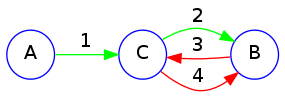
\includegraphics[width=\linewidth,keepaspectratio=true]{broadcast_loop.png}
  \caption{\emph{Broadcast Loops}: Edges are labeled in order of message transmission.  After receiving message 2, node B forwards it back to C as message 3, who will then forward it back to B as message 4 and so on...}
  \label{broadcast_loop}
\end{figure}

Each message, including the originals, will include the ID of the vehicles that witnessed (and participated in) the crash as well as the location of the event in order to facilitate authenticating the information and avoiding the scene, respectively.
Because each vehicle that witnesses the crash begins disseminating messages, there could be a large number of duplicate messages detecting the same event that are treated as distinct for the purposes of forwarding.
This is where data aggregation improves the efficiency of the system.


\subsection{Authenticity \& Aggregation}

In order to enforce authenticity we enforce that each message be signed by a TPM using some form of public key. Each participant in an accident, both victim and witnesses must sign all information regarding accident time and location. When these signatures are collected, an endangered vehicle can make an educated decision depending upon the amount of trust in each message. A message may be untrusted for many reasons, but primarily one may be concerned with an untrustworthy key. Possibly gathered from TPM failure. Thus, a node has the highest level of security when all information from a crash is known. Instead of allowing each original signed message to be disseminated separately, we aggregate them into a single message whenever possible. We rely on signature chaining in order to maintain the same level of trust with just a single message. This technique can be used to aggregate any type of information, not just digital signatures.

Aggregation of this form saves a lot of network overhead by greatly reducing the number of packets that must be transmitted to disseminate the same information.
When a node receives more than one message that pertains to the same crash (as identified by the victim ID), the IDs of the witnesses are combined together into a single packet before forwarding. Along with the ID's the signatures are also forwarded along.
In this way, each packet contains a subset of IDs corresponding to nodes that witnessed or participated in the event, along with their signature of the event specifics.
When a node receives such a packet, it may learn more than one ID as compared to only learning one without any aggregation.

In the case of multiple rebroadcasts, nodes will continuously update the packet they are broadcasting during each interval.
Therefore, if a node learns of another witness, or learns the ID of any crash victim(s), the next packet broadcasted will include this information.
This does not mean that the counter of how many rebroadcasts should be sent is reset, however, as this could prolong the life of the message to a wasteful point.
In this manner, forwarded messages typically contain only one or a small number of IDs initially.
As the message propagates further, aggregation will take place and each message will tend to contain more information about the event.


\section{Simulation and Results}
In this section of the report, we describe the implementation and simulation of the proposed protocol.
We used NS-3 \cite{ns3} to simulate the proposed crash model and measure some performance parameters. A set of classes are integrated with NS-3 to simulate the existence of a highway with several lanes and vehicles driving along them. The mobility model used in our experiment is the \emph{ns3-highway-mobility} model presented in \cite{highway-mobility}.
Vehicles are created and initiated to drive on the highway at a starting point and with some velocity constraints such as minimum and maximum allowed speed. The existing model was very basic with vehicles mostly driving the same speed and on the same lane, which renders it unrealistic. We improved this model by adding some randomness of the vehicles speed limits and allowing them to pass each other by driving on different lanes.

We also added the existence of the crash event. We initialize the simulation with two additional parameters, the crash vehicle and the time of the crash. The first parameter specifies the ID of the vehicle that will crash at a time specified by the second parameter.
When a crash happens, the specified vehicle will stop and send a ``I have crashed'' message and the neighbor vehicles will start disseminating the event information to the rest of the network.
The first message sent by the crash victim is only sent once to model the fact that a serious crash may destroy the vehicle's radio, power source, central computer, etc.

It is worth mentioning that at each time step of the simulation, we write the position of each vehicle and the messages transferred to log files so we can verify the correctness of the implementation.
The vehicle positions log file is used to feed a Java-based tool to vitalize the highway with all the vehicles driving on it during the whole simulation time.
The transferred messages log file, is used to verify the validity of the dissemination and aggregation techniques used in our proposed protocol.
We were able to visualize that the predefined vehicle is really having a crash and all other vehicles are successfully passing it on the road.

\noindent
\begin{figure}[h]
\centering
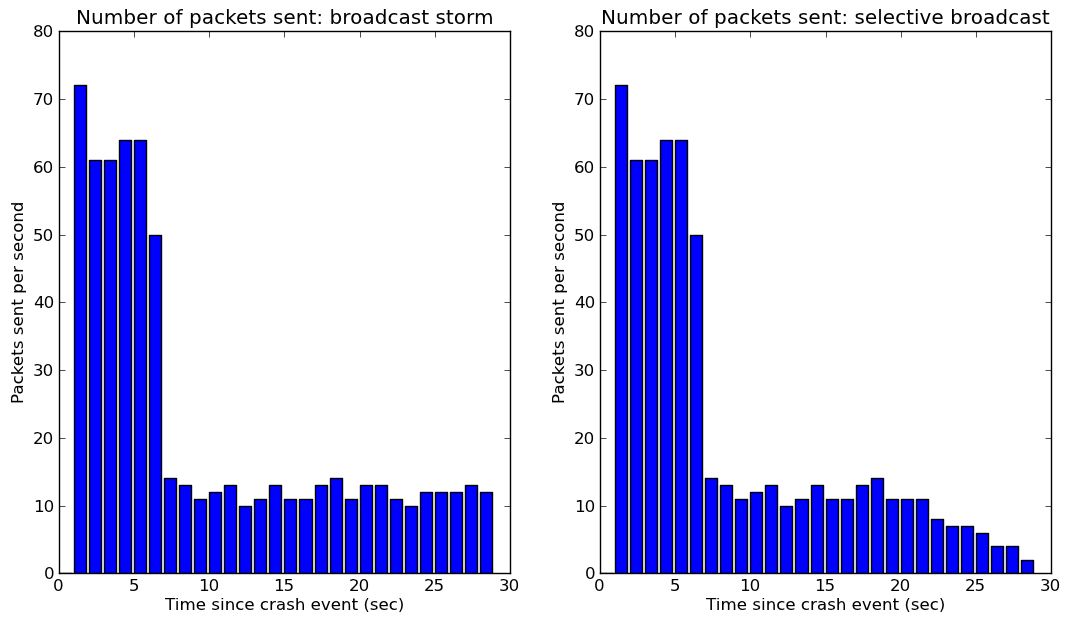
\includegraphics[scale=0.32]{Figure_01.png}
\caption{Broadcast storm versus selective broadcast}
\label{fig_storm_nostorm}
\end{figure}

Figure~\ref{fig_storm_nostorm} shows a comparison between the two cases of using broadcast storm, that is always forwarding a broadcast message even if it has already been seen, and selective broadcast.
We notice that in the case of using selective broadcast, the number of packets transferred in the network starts decreasing after 20 seconds.
The reason is because most vehicles have already received the crash message and start ignoring all message that are already received. On the contrary, vehicles that use broadcast storm keep on forwarding crash messages even if they already received the same messages before.
This explains why after 20 seconds from the crash event, these vehicles continue forwarding messages.

\noindent
\begin{figure}[h]
\centering
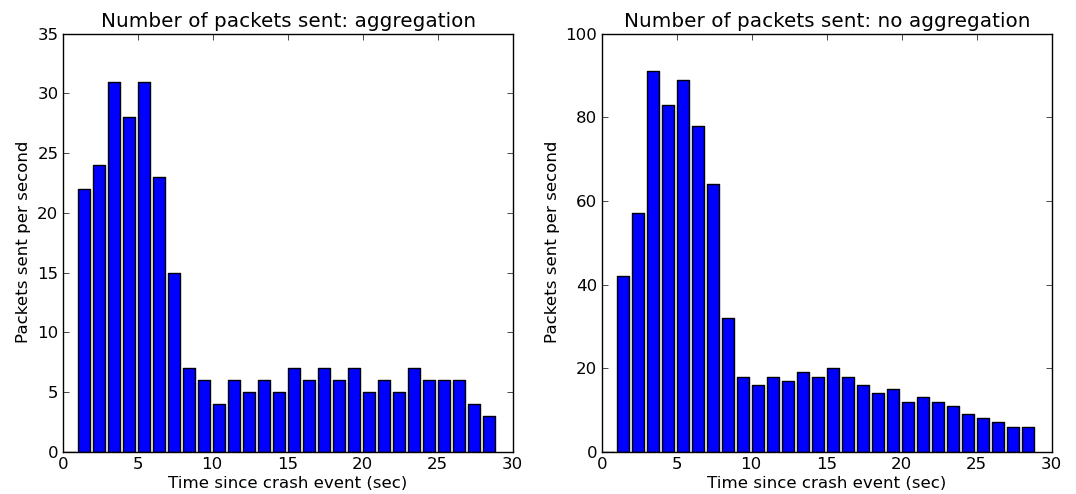
\includegraphics[scale=0.32]{Figure_02.png}
\caption{Aggregation versus non-aggregation}
\label{fig_aggregation_nonaggregation}
\end{figure}

Figure~\ref{fig_aggregation_nonaggregation} illustrates the case where vehicles use aggregation versus not using aggregation.
One can notice that the number of messages sent when aggregation is not present is approximately three times more the number of messages sent when aggregation is used.

\noindent
\begin{figure}[h]
\centering
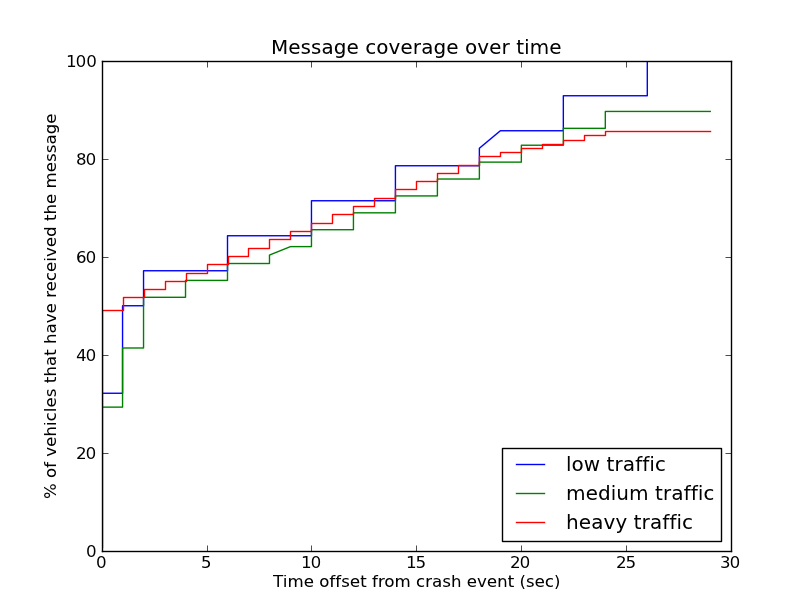
\includegraphics[scale=0.45]{Figure_03.png}
\caption{Message coverage over time}
\label{fig_msg_coverage}
\end{figure}

In Figure~\ref{fig_msg_coverage}, we demonstrate the different dissemination patterns when low, medium and heavy traffic are present.
It shows that after roughly $25$ seconds of simulation, all of the vehicles that are suppose to have received the crash message already have.
At time $0$ seconds, or right after the crash occurs, we notice that $50\%$ of the vehicles have received the crash message in the heavy traffic case whereas only $30\%$ of them received the message in low and medium traffic.
It is worth mentioning that the vehicles receiving the messages are the ones that are close to the crash area which means that the more recipients there are, the better the locality of the dissemination.
As time progresses, the message coverage curves for the three traffic density cases start the converge together.
Moreover, it can be noticed that the cases where heavy traffic exists have smoother message coverage curve due to the presence of a lot of vehicles close to each others.
Thus vehicles carrying the message do not need to travel for very long before coming into the vicinity of other vehicles to transfer the message to.

\section{Conclusion}

In this paper, we proposed a secure method for quickly aggregating and disseminating information about crash events in VANETs.
The protocol was implemented in a simulation environment to show its efficacy.
We determined that our method is effective at reaching all local nodes very quickly even in a variety of traffic conditions.
By extending the ns3-highway-mobility project, we have also furthered VANET simulation research as our modifications are publicly available for others to benefit from.
To conclude the paper, we discuss some optimizations and possible future work as well as alternative applications for our protocol.

\subsection{Optimizations and Future Work}

Although we did not have time to implement them, we considered a few optimizations and extensions to our protocol.
One involved adapting the forwarding and re-broadcasting mechanism to the number and location of other nodes nearby.
If a node is located within the center of a node cluster that it knows has already received a message, by overhearing each of them broadcast the message or an acknowledgement of it, it does not need to rebroadcast the message itself as it will not reach any additional nodes that the others cannot already.
This could prevent some excess broadcasts and reduce the load on the network, although it would add a large degree of complexity to the protocol and require careful negotiation between the nodes.
Not only would each node need to keep track of what nodes around it have received the message, it must also know that there are no other nodes present that have not yet.
This could be accomplished by overhearing other protocols that would likely be utilized in VANETs, such as range-finding and movement negotiations.
However, it is still difficult to say with certainty whether another node has entered one's broadcast radius or not.

We also considered adjusting the time between rebroadcasts, and even the actual number of rebroadcasts, based on the local node density of the network, and the proximity to the crash event.
Our simulation results indicate that event data can be disseminated far quicker with higher traffic densities due to the decreased space between each vehicle.
This indicates that some parameters might be relaxed in order to decrease the number of messages in the network and frequency of rebroadcasting while still maintaining the same dissemination speed.

Although we did not consider utilizing dedicated infrastructure in our system, it could certainly be used for improvements.
If a VANET-equipped road has a series of radio towers along it to aid communication between the vehicles, they could be used to more rapidly spread information without adding load to wireless channel.
By using higher-powered road-side antennae, each tower could cover more vehicles in a shorter amount of time than ad-hoc communications.
Furthermore, the towers could pass the message further back the road to reach vehicles coming towards the crash by communicating with each other either wirelessly or through a wired link.
A cellular network could be used in a similar manner, although, as previously discussed, the latency on cellular towers makes them less suitable for our particular application.
Even so, they might be used to notify a large area of vehicles about the event and perhaps stop the ad-hoc dissemination of it once the dedicated infrastructure becomes aware and can take over the dissemination process.
A combination of all three (ad-hoc, road-side, and cellular) networks may also prove to be the most effective and flexible when properly managed.

\subsection{Other Applications}

While our technique was intended for detection of and notification about crash events in VANETs, it could be applied in other domains as well.
For example, it could be used for notification of other impending hazards, such as road debris, weather, or simply traffic congestion.
Some modifications to the protocol details could make it suitable for exchanging basic information as well.
For example, our method of aggregating messages could be used to efficiently determine the approximate speed of traffic and negotiate which vehicles should be in which lane and how fast for them to travel.
It could also be used to notify very close vehicles (perhaps with a TTL of 2 or 3 hops) about one's intentions, such as changing lanes or making turns.

In addition to VANETs, this protocol might be applied in other areas, such as wireless sensor networks.
Indeed, we discussed how data aggregation is often used in this domain, especially for the purpose of reducing power consumption.
One can envision a system in which sensor devices and/or sinks only have intermittent connections, either due to movement or perhaps powering down their radios and only periodically coming on-line to listen for any interesting data.
In this case, the application of staggered repeated broadcasts may help ensure data delivery and even reduce power consumption if the nodes effectively coordinated.

Outside of the wireless domain, our protocol might find use in a peer-to-peer system.
By using the technique of staggered rebroadcasting, peers might send some important information to nodes that either join the network or move around within it.
This could help to address the issue of churn that is so common in these systems, ensuring that each node is aware of the pertinent data and allowing them to more efficiently distribute it as more pieces become known through aggregation.


\bibliographystyle{IEEEtran}
\bibliography{project_report}
\end{document}
